% Use the standalone as the document class with an option which allows specifying the border.
\documentclass[border = 10pt]{standalone}

% Allow to entering comfortably English.
\usepackage[T1]{fontenc}
\usepackage[utf8]{inputenc}
\usepackage[french]{babel}

% 
\usepackage{xcolor}
\definecolor{color0}{HTML}{372639}
\definecolor{color1}{HTML}{C2A4C0}
\definecolor{color2}{HTML}{816288}
\definecolor{color3}{HTML}{C6926C}
\definecolor{color4}{HTML}{D5BEA9}
\definecolor{color5}{HTML}{DBCAD3}


%
\usepackage{tikz}
%
\usetikzlibrary{mindmap}
%
\usetikzlibrary{shadows}

\usepackage[hidelinks, pdfencoding = auto]{hyperref}

\usetikzlibrary{backgrounds}

\usepackage{wallpaper}

\begin{document}
	
\ThisCenterWallPaper{}{./figures/Social_Network_Analysis_Visualization_transparent.png}

\centering

\begin{tikzpicture}

\begin{scope}
	[
		mindmap,
		every node/.style =
		{
			concept,
			execute at begin node = \hskip 0pt
		},
		root concept/.append style =
		{
			concept color = color0,
			rectangle,
			rounded corners = 2em,
			fill = color5!10,
			line width = 0.5em,
			text width = 40em,
			text = color0,
			font = \huge\scshape,
			inner sep = 2em
		}
	]
	\node [root concept] (Nom de projet)
	at (0em, 0em) {{Federated Machine Learning}};
\end{scope}

\begin{scope}
	[
		mindmap,
		text = color0,
		grow cyclic,
		every node/.style =
			{
				concept,
				concept color = color1!50,
				text = color0,
				execute at begin node = \hskip 0pt
			},
		root concept/.append style =
			{
				concept color = color1,
				draw = color1!75,
				fill = color1!10,
				line width = 1em,
				text width = 20em,
				text = color0,
				font = \LARGE\scshape,
				inner sep = 0pt
			},
		level 1/.append style =
			{
				concept color = color1,
				draw = color1!50,
				fill = color1!5,
				line width = 0.5em,
				text width = 18em,
				text = color0,
				font = \Large\bfseries,
				inner sep = 0pt
			},
		level 2/.append style =
			{
				concept color = color1,
				draw = color1!50,
				fill = color1!5,
				line width = 0.5em,
				text width = 16em,
				text = color0,
				font = \large\bfseries,
				inner sep = 0pt
			},
		level 3/.append style =
		{
			concept color = color1,
			rectangle,
			draw = color1!50,
			fill = color1!5,
			line width = 0.5em,
			text width = 16em,
			text = color0,
			font = \large\bfseries,
			inner sep = 0pt
		}
	]

	\node [root concept, text width = 20em, inner sep = 1em] (APERÇU)
		at (-120em, 60em)
			{\LARGE{APERÇU DE \\L'APPRENTISSAGE \\FÉDÉRÉ}}
		child [grow = 90, level distance = 30em, concept color = color1!50]
			{
				node [level 1, text width = 18em, inner sep = 1em] (L'idée principale) {\Huge\textsc{L'idée principale}}
				child [grow = 45, level distance = 30em, concept color = color1!50]
				{
					node [level 2, text width = 16em, inner sep = 1em] (L'idée principale - 1) {\huge{créer des \\modèles \\d'apprentissage}}
					child [grow = 45, level distance = 30em, concept color = color1!50]
					{
						node [level 3, text width = 20em, inner sep = 2em] (L'idée principale - 1 - 1) {\LARGE{basés sur \\des données réparties \\sur plusieurs appareils}}
					}
				}
				child [grow = 90, level distance = 30em, concept color = color1!50]
				{
					node [level 2, text width = 16em, inner sep = 1em] (L'idée principale - 2) {\huge{prévenir les fuites de données}}
				}
		 	}
		child [grow = 150, level distance = 30em, concept color = color1!50]
			{
				node [level 1, text width = 18em, inner sep = -1em] (Les améliorations concentrées) {\huge\textsc{Les \\améliorations \\concentrées}}
				child [grow = 90, level distance = 30em, concept color = color1!50]
				{
					node [level 2, text width = 16em, inner sep = 1em] (Les améliorations concentrées - 1) {\huge{la résolution \\des défis \\statistiques}}
				}
				child [grow = 130, level distance = 30em, concept color = color1!50]
				{
					node [level 2, text width = 16em, inner sep = 1em] (Les améliorations concentrées - 2) {\huge{l'amélioration \\de la sécurité \\dans \\l'apprentissage \\fédéré}}
				}
				child [grow = 170, level distance = 30em, concept color = color1!50]
				{
					node [level 2, text width = 16em, inner sep = 1em] (Les améliorations concentrées - 3) {\huge{rendre \\l'apprentissage \\fédéré plus \\personnalisable}}
				}
			}
		child [grow = -150, level distance = 30em, concept color = color1!50]
		{
			node [level 1, text width = 18em, inner sep = -1em] (Définition de l'apprentissage fédéré) {\huge\textsc{Définition de \\l'apprentissage \\fédéré}}
			child [grow = 150, level distance = 30em, concept color = color1!50, densely dashed]
			{
				node [level 2, text width = 16em, inner sep = 1em] (Définition de l'apprentissage fédéré - 1) {\huge{la méthode \\conventionnelle}}
				child [grow = 165, level distance = 40em, concept color = color1!50]
				{
					node [level 3, text width = 20em, inner sep = 2em] (Définition de l'apprentissage fédéré - 1 - 1) {\huge{rassembler \\toutes les données}}
				}
				child [grow = 180, level distance = 40em, concept color = color1!50]
				{
					node [level 3, text width = 30em, inner sep = 2em] (Définition de l'apprentissage fédéré - 1 - 2) {\huge{utiliser $D = {D}_{1}\cup...\cup{D}_{N}$ \\pour former un modèle ${M}_{SUM}$}}
				}
			}
			child [grow = 190, level distance = 30em, concept color = color1!50]
			{
				node [level 2, text width = 16em, inner sep = 1em] (Définition de l'apprentissage fédéré - 2) {\huge{un processus \\d'apprentissage}}
				child [grow = 165, level distance = 40em, concept color = color1!50]
				{
					node [level 3, text width = 28em, inner sep = 2em] (Définition de l'apprentissage fédéré - 2 - 1) {\huge{les propriétaires de données \\forment en collaboration \\un modèle ${M}_{FED}$}}
				}
				child [grow = 180, level distance = 40em, concept color = color1!50]
				{
					node [level 3, text width = 34em, inner sep = 2em] (Définition de l'apprentissage fédéré - 2 - 2) {\huge{aucun propriétaire de données ${F}_{i}$ \\n'expose ses données ${D}_{i}$ à d'autres}}
				}
			}
			child [grow = 230, level distance = 30em, concept color = color1!50]
			{
				node [level 2, text width = 16em, inner sep = 1em] (Définition de l'apprentissage fédéré - 3) {\LARGE{$\left| {V}_{FED} - {V}_{SUM}\right| < \delta$}}
				child [grow = 180, level distance = 40em, concept color = color1!50]
				{
					node [level 3, text width = 24em, inner sep = 2em] (Définition de l'apprentissage fédéré - 3 - 1) {\huge{${V}_{FED}$, \\la précision de ${M}_{FED}$}}
				}
				child [grow = 205, level distance = 40em, concept color = color1!50]
				{
					node [level 3, text width = 26em, inner sep = 2em] (Définition de l'apprentissage fédéré - 3 - 2) {\huge{${V}_{SUM}$, \\la performances de ${M}_{SUM}$}}
				}
				child [grow = -90, level distance = 25em, concept color = color1!50]
				{
					node [level 3, text width = 42em, inner sep = 2em] (Définition de l'apprentissage fédéré - 3 - 3) {\huge{$\delta$, un nombre réel non négatif, \\perte de précision d'apprentissage fédéré}}
				}
			}
		}
		child [grow = -90, level distance = 30em, concept color = color1!50]
		{
			node [level 1, text width = 18em, inner sep = -1em] (Confidentialité de l'apprentissage fédéré) {\huge\textsc{Confidentialité \\de \\l'apprentissage \\fédéré}}
			child [grow = -145, level distance = 30em, concept color = color1!50]
			{
				node [level 2, text width = 16em, inner sep = 1em] (Confidentialité de l'apprentissage fédéré - 1) {\huge{1. calcul \\multiparties \\sécurisées \\(SMC)}}
			}
			child [grow = -90, level distance = 30em, concept color = color1!50]
			{
				node [level 2, text width = 16em, inner sep = 1em] (Confidentialité de l'apprentissage fédéré - 2) {\huge{2. confidentialité \\différentielle}}
			}
			child [grow = -45, level distance = 30em, concept color = color1!50]
			{
				node [level 2, text width = 16em, inner sep = 1em] (Confidentialité de l'apprentissage fédéré - 3) {\LARGE{3. cryptage homomorphe}}
			}
			child [grow = 0, level distance = 30em, concept color = color1!50]
			{
				node [level 2, text width = 16em, inner sep = 1em] (Confidentialité de l'apprentissage fédéré - 4) {\LARGE{une des propriétés \\essentielles de \\l'apprentissage \\fédéré}}
			}
		}
		child [grow = 0, level distance = 30em, concept color = color1!50]
		{
			node [level 1, text width = 18em, inner sep = -1em] (Catégorisation de l'apprentissage fédéré) {\huge\textsc{Catégorisation \\de \\l'apprentissage \\fédéré}}
			child [grow = 0, level distance = 40em, concept color = color1!50]
			{
				node [level 2, text width = 30em, inner sep = 2em] (Catégorisation de l'apprentissage fédéré - 1) {\huge{matrice ${D}_{i}$ dénote \\les données de propriétaire {i} \\chaque ligne représente \\un échantillon \\chaque colonne représente \\une caractéristique}}
				child [grow = 90, level distance = 45em, concept color = color1!50]
				{
					node [level 3, text width = 30em, inner sep = 1em] (Catégorisation de l'apprentissage fédéré - 1 - 1) {\LARGE\textsc{Apprentissage fédéré horizontal}\\
						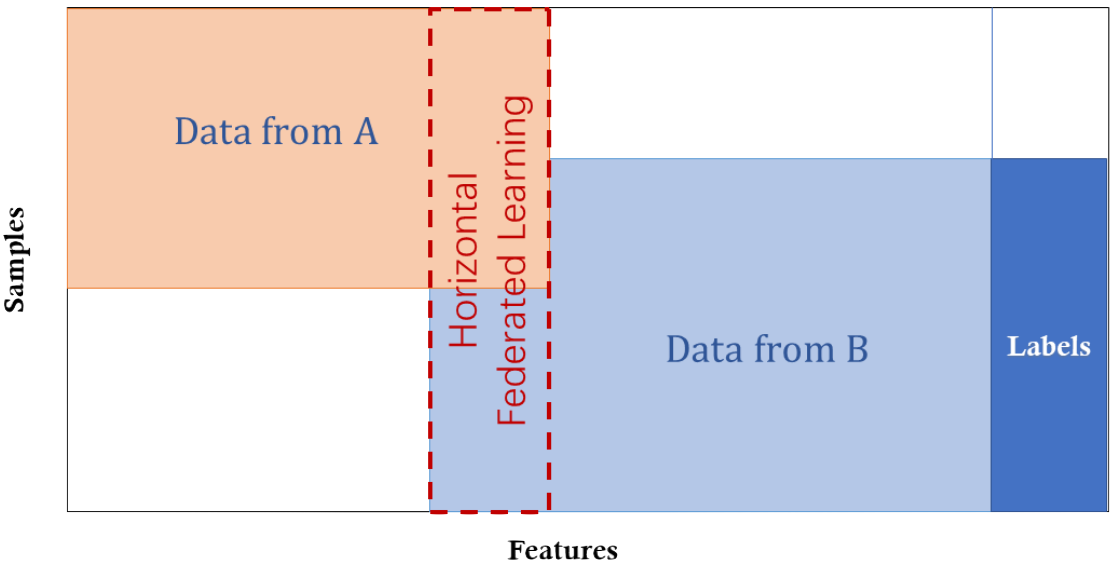
\includegraphics[width = 1\textwidth]{./figures/Figure 1.png}}
				}
				child [grow = 0, level distance = 50em, concept color = color1!50]
				{
					node [level 3, text width = 30em, inner sep = 1em] (Catégorisation de l'apprentissage fédéré - 1 - 2) {\LARGE\textsc{Apprentissage fédéré vertical}\\
						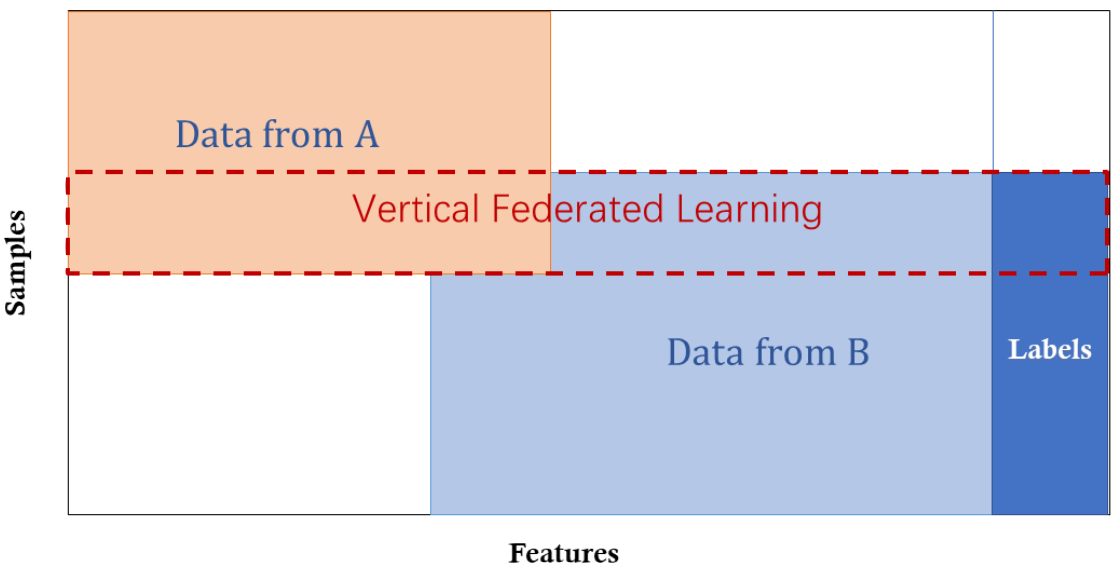
\includegraphics[width = 1\textwidth]{./figures/Figure 2.png}}
				}
				child [grow = -90, level distance = 45em, concept color = color1!50]
				{
					node [level 3, text width = 30em, inner sep = 1em] (Catégorisation de l'apprentissage fédéré - 1 - 3) {\LARGE\textsc{Apprentissage par transfert fédéré (FTL)}\\
						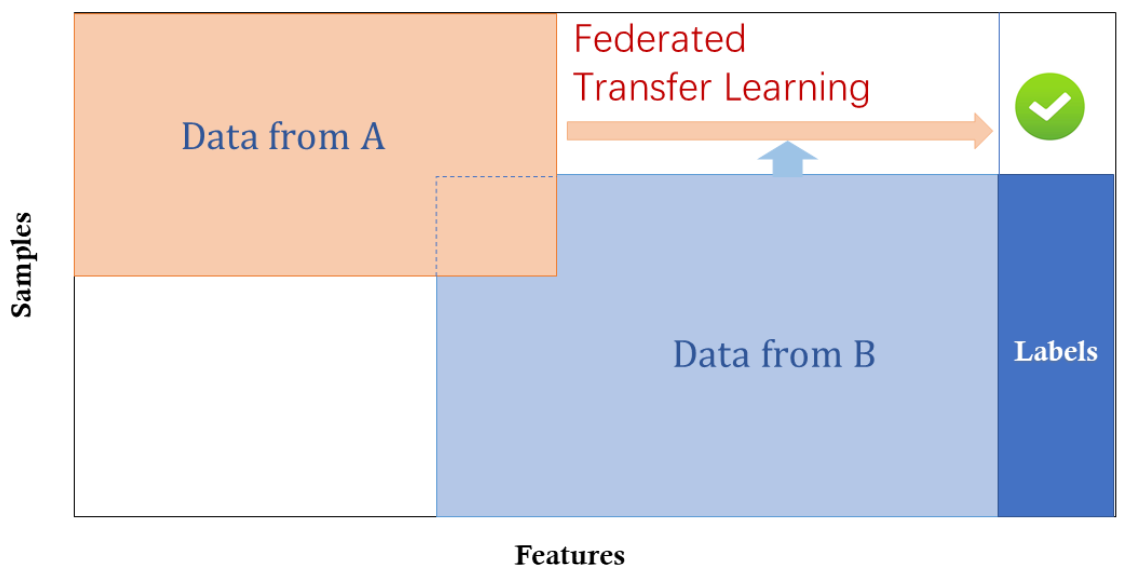
\includegraphics[width = 1\textwidth]{./figures/Figure 3.png}}
				}
			}
		}
	; 
	\begin{pgfonlayer}{background}
		\draw [densely dashed] 
			;
	\end{pgfonlayer}
\end{scope}

\end{tikzpicture}

\end{document}
